\chapter{評価実験}
\thispagestyle{fancy}


\section{評価方法}
図\ref{kankyou}のようにプロジェクターとKinectを配置する.
体験者はKinectの正面に立つ.
本研究で提案したプロジェクションマッピングを5名に体験してもらい,
評価を得るためにアンケートを実施した.

\vspace{1cm}
\begin{figure}[h]
  \centering
  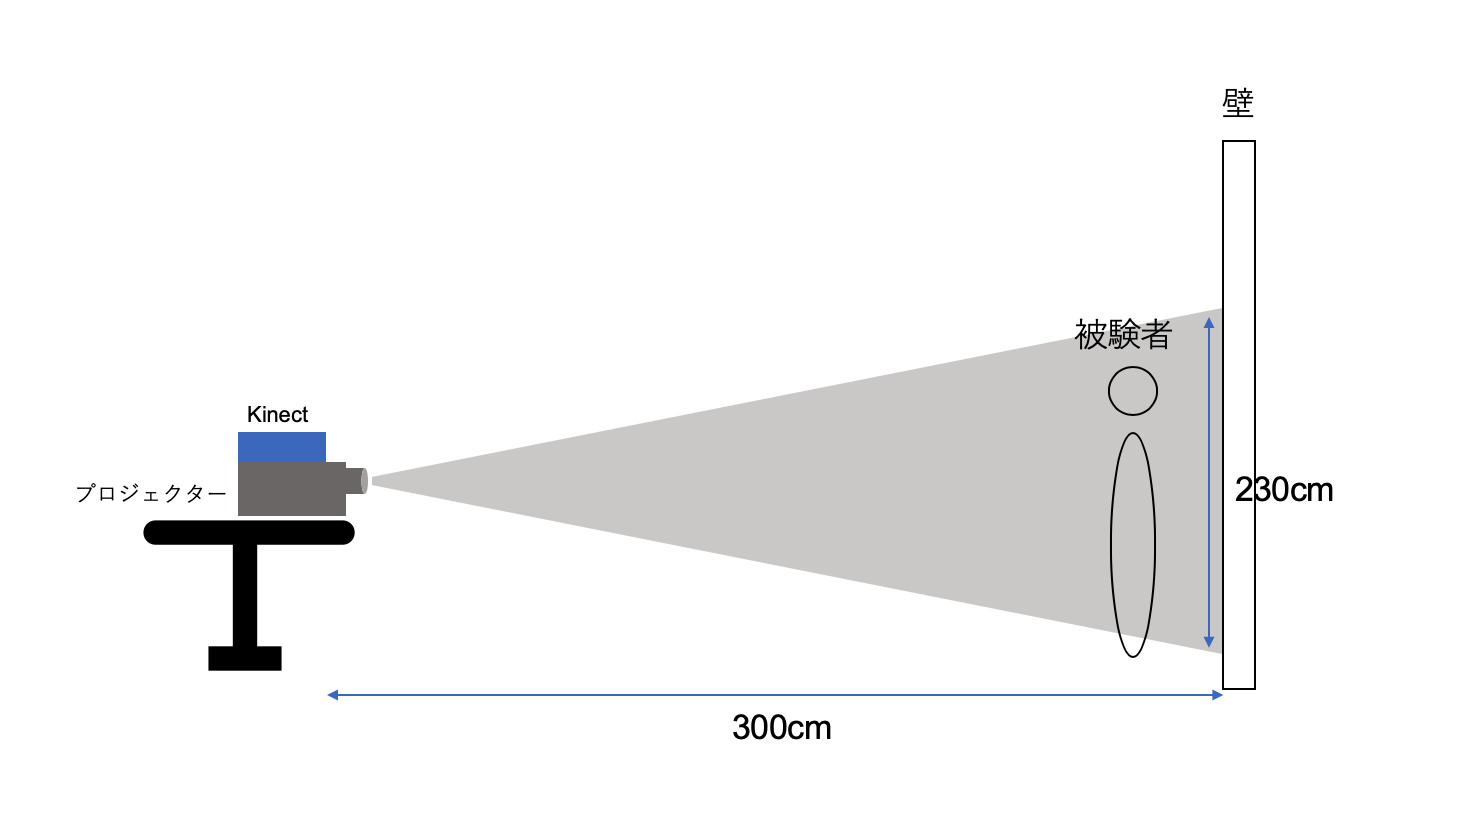
\includegraphics[width=14cm]{image/jikkenkankyou.png}
  \caption[評価実験環境図]{評価実験環境図.}
\label{kankyou}
\end{figure}


\clearpage

アンケートの質問内容を以下に示す.
\begin{itemize}
  \item[Q1.] 操作はわかりやすいか? [5段階評価]
  \item[Q2.] わかりづらかった場合,どこがわかりづらいか? 
  \item[Q3.] 楽しさについての満足感はどれくらいか? [5段階評価]
  \item[Q4.] 今後の改善点や意見・要望   
\end{itemize}



\section{評価結果}
図\ref{hyouka}にアンケート結果を示す.

Q1の操作わかりやすさに関しては平均4となった.

Q2のわかりにくかった部分の回答では「操作方法が口頭での説明だったので教えてもらうまでわからなかった.」
という回答が得られた.


\vspace{1cm}
\begin{figure}[h]
  \centering
  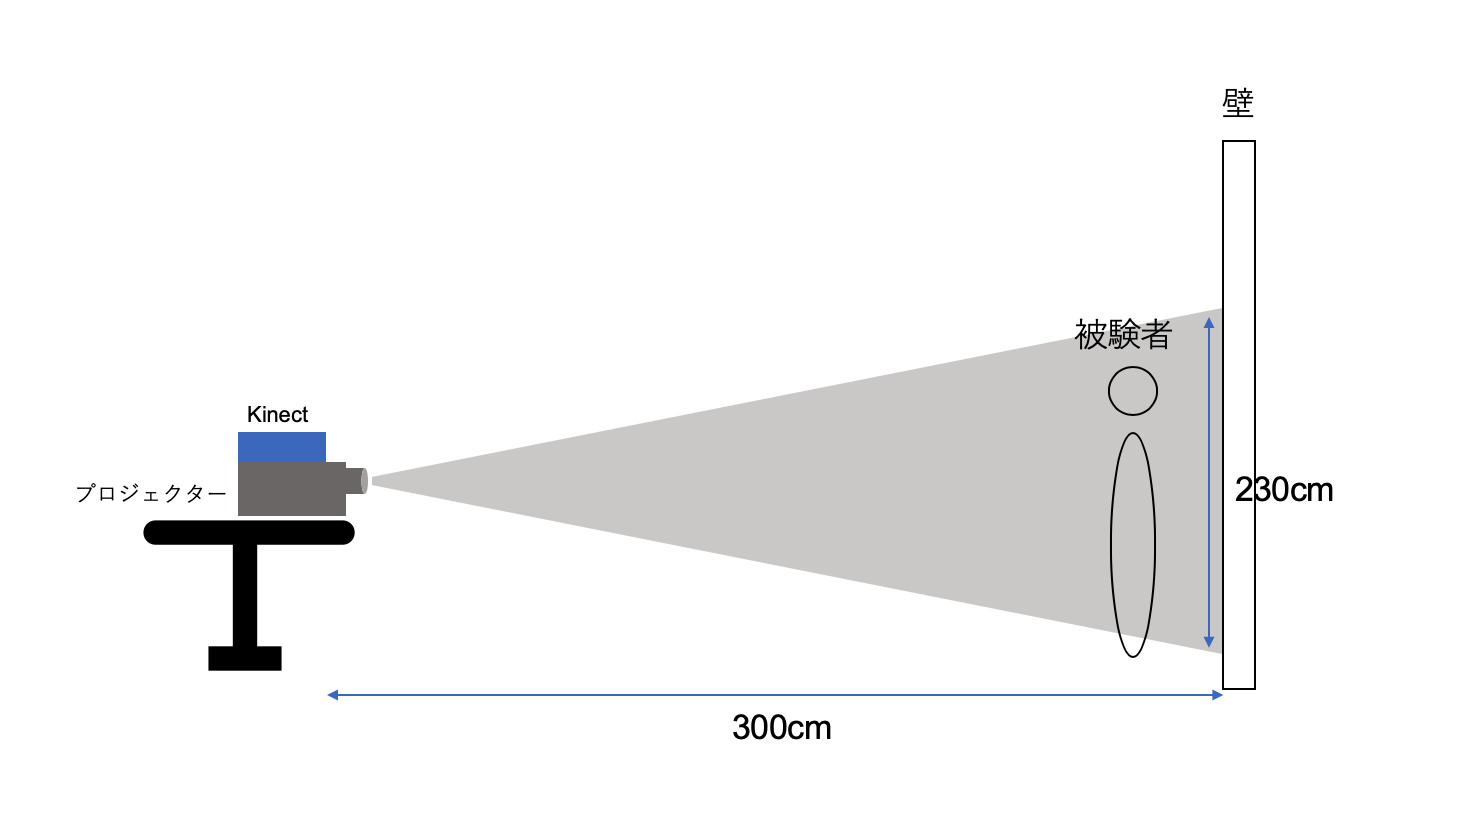
\includegraphics[width=7cm]{image/jikkenkankyou.png}
  \caption[評価実験環境図]{評価実験環境図.}
\label{hyouka}
\end{figure}
